\documentclass[11pt]{article}

\usepackage[utf8]{inputenc}
\usepackage{tabularx}
\usepackage{hyperref}
\usepackage{array}  
\usepackage{graphicx}
\usepackage{geometry} 
\usepackage{fancyhdr} 
\usepackage{tikz}
\usepackage{ragged2e}
\usepackage{anyfontsize}
\usepackage[table,xcdraw]{xcolor}
\usepackage{tabularx, etoolbox} 
\usepackage{eso-pic}
\usepackage{float}
\usepackage{longtable}

\graphicspath{{images}}
%\graphicspath{{../images/}}

\setcounter{secnumdepth}{4}


%cambio misure della pagina
\geometry{a4paper,left=25mm,right=25mm,top=25mm,bottom=25mm}
%ebdfc7
\definecolor{colorePie}{HTML}{ebdfc7}
\pagestyle{fancy}
\fancyhf{}
\renewcommand{\headrulewidth}{0.4pt}
\lhead{
    \parbox[c]{1cm}{\includegraphics[width=1.1cm]{Sevenbitslogo.png}}
}
\rhead{\textcolor[HTML]{9e978a}{ ANALISI DEI REQUISITI v0.5.0}
}
\setlength{\headheight}{25pt}
\cfoot{\thepage}


\renewcommand*\contentsname{Indice}
\renewcommand{\listfigurename}{Elenco delle figure}
\renewcommand{\listtablename}{Elenco delle tabelle}

\begin{document}

% Pagina del titolo
\begin{titlepage}
    \setcounter{page}{0}
    \centering
    % Inserisci il logo del gruppo (modifica il percorso dell'immagine)
    \includegraphics[width=7.2cm]{Sevenbitslogo.png} \\[2cm] 
    
    % Titolo
     {\fontsize{40}{40}\bfseries Analisi dei Requisiti}\selectfont \\[3.9em]
    
    % Sottotitolo
    {\huge NearYou\\ \vspace{3mm }Smart custom advertising platform} \\[2.7em]
    
    % Email del gruppo
    {\large sevenbits.swe.unipd@gmail.com} \\[3em]
    
    % Spazio per il logo dell'università
    \hfill
      
    \AddToShipoutPictureBG{ % Imposta il triangolo con logo
        \ifnum\value{page}=0
        \begin{tikzpicture}[overlay]
        
            % Definisce un triangolo blu in basso a destra
            \fill[colorePie] 
                (current page.south east) -- ++(-9cm,0) -- ++(9cm,9cm);
            
            % Inserisce il logo all'interno del triangolo
            \node[anchor=south east, xshift=-0.3cm, yshift=0.3cm] at (current page.south east) {
                \includegraphics[width=4.5cm]{LogoUnipd.png}
            };
        \end{tikzpicture}
        \fi
    }
        
\vfill % Aggiunge spazio verticale per centrare il contenuto
\end{titlepage}
\newpage
\clearpage
\setcounter{page}{1}

\centering\textbf{Registro modifiche}\\
\vspace{2mm}
\begin{tabularx}{\textwidth}{|l|l|l|l|X|}
\hline
\textbf{Versione} & \textbf{Data} & \textbf{Autore} & \textbf{Verificatore} & \textbf{Descrizione} \\
\hline
0.5.2 & 2025-01-14 & Manuel Gusella & Alfredo Rubino & Modifica RF18 e RF19 dopo modifica\\
\hline
0.5.1 & 2025-01-13 & Manuel Gusella & Federico Pivetta & Modifica di \hyperref[UC7]{UC7},\hyperref[UC8]{UC8},\hyperref[UC9]{UC9}, \hyperref[UC10]{UC10} e \hyperref[UC11]{UC11} e RF02\\
\hline
0.5.0 & 2025-01-6 & Uncas Peruzzi & Riccardo Piva & Aggiunta di \hyperref[UC10]{UC10}, \hyperref[UC11]{UC11} e \hyperref[UC12]{UC 12}\\
\hline
0.4.0 & 2025-01-5 & Uncas Peruzzi & Riccardo Piva & Aggiunta di \hyperref[UC7]{UC7}, \hyperref[UC8]{UC8} e \hyperref[UC9]{UC 9}\\
\hline
0.3.0 & 2025-01-4 & Uncas Peruzzi & Riccardo Piva & Refactoring generale casi d'uso esistenti\\
\hline
0.2.10 & 2024-12-27 & Manuel Gusella & Riccardo Piva & Fine stesura \hyperref[UC1.1]{UC 1.1}, cambiamenti marginali agli \hyperref[UC1.2]{UC 1.2} e \hyperref[UC1.3]{UC 1.3} e stesura \hyperref[UC6]{UC 6} e RF13\\
\hline
0.2.9 & 2024-12-24 & Manuel Gusella & Uncas Peruzzi & Aggiunta di \hyperref[UC1.1.1]{UC 1.1.1} e RF12, cambiamento \hyperref[UC1.1]{UC1.1} \\
\hline
0.2.8 & 2024-12-24 & Manuel Gusella & Riccardo Piva & Aggiunta di \hyperref[UC1.2.1]{UC 1.2.1} e RF11, aggiustamento \hyperref[UC1.3.2]{UC1.3.2} \\
\hline
0.2.7 & 2024-12-02 & Manuel Gusella & Giovanni Cristellon & Aggiunta di UC1.3.2 e RF10 \\
\hline
0.2.6 & 2024-11-30 & Federico Pivetta & Giovanni Cristellon & Aggiunta di RQ05, RQ06, RV05, RP02, indice tabelle e nuovo stile tabelle \\
\hline
0.2.5 & 2024-11-29 & Uncas Peruzzi & Leonardo Trolese & Aggiunta di UC5, aggiornati Requisiti$_G$ di qualità, vincolo e tabella \\
\hline
0.2.4 & 2024-11-28 & Federico Pivetta & Leonardo Trolese & Aggiunta di UC1.3, UC1.3.1, RF02, RF04 e RF05, correzione tabella Requisiti$_G$ funzionali \\
\hline
0.2.3 & 2024-11-26 & Leonardo Trolese  & Federico Pivetta & Correzioni minori grammaticali e di contenuto \\
\hline
0.2.2 & 2024-11-25 & Leonardo Trolese  & Federico Pivetta & Aggiunta di UC3, UC3.1, UC3.2, UC4, RF01 e RF08 \\
\hline
0.2.1 & 2024-11-23 & Manuel Gusella  & Federico Pivetta & Aggiunta di UC1.2, UC2, RF03 e RF06\\
\hline
0.2.0 & 2024-11-21 & Uncas Peruzzi  & Federico Pivetta & Migliorie varie e inizio redazione sez.\ref{sec:casi-uso} \\
\hline
0.1.1 & 2024-11-15 & Uncas Peruzzi  & Riccardo Piva & Redazione sez.\ref{sec:intro} e sez.\ref{sec:descrizione} \\
\hline
0.1.0 & 2024-11-14 & Uncas Peruzzi  & Riccardo Piva & Inizio redazione del documento\\
\hline
\end{tabularx}

\newpage
\tableofcontents
\newpage
\listoffigures
\newpage
\listoftables

\newpage
\begin{justify}

\section{Introduzione}
\label{sec:intro}

\subsection{Scopo del documento}

Il seguente documento ha l'obiettivo di fornire una descrizione accurata dei Casi-d'uso$_G$ e dei Requisiti$_G$ riguardanti il Progetto$_G$ \textit{"NearYou - 
Smart custom advertising platform"} concernenti il Capitolato$_G$ C4 proposto dall'azienda Synclab$_G$ e aggiudicato al gruppo dal Committente$_G$.


\subsection{Glossario}
Con l'intento di evitare ambiguità interpretative del linguaggio utilizzato, viene fornito un Glossario che si occupa di esplicitare il significato dei termini che riguardano il contesto del Progetto$_G$. I termini presenti nel glossario sono contrasegnati con una \textit{G} a pedice : Termine$_G$.\\
Le definizioni sono presenti nell'apposito documento \textit{Glossario.pdf}


\subsection{Riferimenti}

\subsubsection{Riferimenti normativi}
\begin{itemize}
    \item[-] ISO/IEC/IEEE 29148:2018(E) \\
    \textcolor{blue}{\texttt{\url{https://ieeexplore.IEEE.org/stamp/stamp.jsp?tp=&arnumber=8559686}}}
    
    \item[-] Regolamento del Progetto$_G$ didattico  \\
    \textcolor{blue}{\texttt{\url{https://www.math.unipd.it/~tullio/IS-1/2024/Dispense/PD1.pdf}}}
    
\end{itemize}
\subsubsection{Riferimenti informativi}
\begin{itemize}
    \item[-] Capitolato$_G$ C4 - NearYou - Smart custom advertising platform\\
    \textcolor{blue}{\texttt{\url{https://www.math.unipd.it/~tullio/IS-1/2024/Progetto$_G$/C4p.pdf}}}
    \item[-] Analisi-dei-Requisiti$_G$ - SWE 2024-25\\
    \textcolor{blue}{\texttt{\url{https://www.math.unipd.it/~tullio/IS-1/2024/Dispense/T05.pdf}}}
    \item[-] Analisi e descrizione delle funzionalità: Use Case e relativi diagammi - SWE 2024-25\\    
    \textcolor{blue}{\texttt{\url{https://www.math.unipd.it/~rcardin/swea/2022/Diagrammi\%20Use\%20Case.pdf}}}
    \item[-] Verbali Interni
    \item[-] Verbali Esterni
    
\end{itemize}

\newpage
\section{Descrizione del prodotto}
\label{sec:descrizione}
\subsection{Obiettivi del prodotto}
Il prodotto software da sviluppare, ha il principale obiettivo di generare annunci personalizzati per l'utente, sulla base della sua profilazione e posizione in tempo reale sulla mappa, tramite l'utilizzo degli LLM$_G$, nel momento in cui si trovi su un veicolo (dotato di display). Il risultato desiderato, prevede di proporre agli utenti esclusivamente annunci finalizzati a catturare il loro interesse, con il fine di massimizzare il tasso di engagement.

\subsection{Ambito del prodotto}
Il campo di applicazione del prodotto software \textit{NearYou - 
Smart custom advertising platform}, è focalizzato su una serie di clienti che offrono un servizio di renting di mezzi di trasporto, dotati di display, nei quali durante l'itinerario di viaggio vengano presentate pubblicità mirate in base a diversi fattori:
\begin{itemize}
    \item [-] sensori di posizione (GPS);
    \item [-] informazioni date dagli utenti in fase di iscrizione;
    \item [-] informazioni di stato fisico dell’utente.
\end{itemize}

\subsection{Panoramica del prodotto}
\subsubsection{Prospettiva generale del prodotto} 
In questa sezione vengono elencate tutte le interfacce di sistema che possono interagire con il prodotto \textit{Near You}.

\paragraph{Interfacce utente}\mbox{}\\
\textit{Near You} è un prodotto che genera messaggi pubblicitari personalizzati per l'utente. Questi messaggi sono pensati per essere visualizzati mediante un'interfaccia utilizzabile su display touchscreen, con la quale l'utente può interagire visivamente e fisicamente; tuttavia con la Proponente$_G$ è stato stabilito che tale interfaccia utente 
è un Requisito$_G$ opzionale poiché può essere facilmente ottenuta a partire dalla Dashboard$_G$ dell'utente privilegiato mediante un semplice filtro.\\
In ogni caso, nell'ambiente di sviluppo del prodotto, il display è emulato tramite una web-app che presenta una mappa interattiva sulla quale vengono visualizzate pubblicità associate ai punti di interesse. Per l'utente 
privilegiato, che offre il servizio di renting, è invece presente, come accennato prima, una Dashboard$_G$ nella quale è possibile visualizzare la mappa, con tutte le posizioni live dei mezzi e i vari punti di interesse, 
generati dal software sottostante.

\paragraph{Interfacce hardware}\mbox{}\\
Il prodotto sviluppato sfrutta i dati monitorati e acquisiti da sensori, nel contesto di sviluppo saranno dati generati attraverso simulazioni reali. Il display touchscreen, corrisponderà a una web-app accessibile da un web browser.\\
Come risultato di quanto detto lo sviluppo del Progetto$_G$ non avviene con elementi hardware fisici.

\subsubsection{Funzionalità del prodotto}
Il prodotto software dovrà garantire le seguenti caratteristiche:
\begin{itemize}
    \item [-] generazione e salvataggio di dati personali relativi a utenti fittizi, su cui dimostrare il funzionamento del software.
    \item [-] simulazione dati provenienti dai sensori GPS, nel caso del percorso effettuato dall'utente, deve corrispondere a coordinate di itinerari che esistono realmente.
    \item [-] separazione del flusso di dati generato dai simulatori, tramite l'utilizzo di un broker opportuno, facilitando di fatto la gestione delle informazioni tra i diversi componenti del sistema.
    \item [-] individuazione dei punti di interesse specifici, sfruttando LLM$_G$, che prende in input i dati di profilazione e posizione simulati.
    \item [-] serializzazione dei dati precedentemente menzionati, in un Database$_G$ adatto alla tipizzazione degli input e performante in tale contesto.
    \item [-] acquisizione e elaborazione dei dati dei sensori per mezzo di uno strumento adatto allo stream processing, per fornirli in pasto al framework$_G$ di generative AI.
    \item [-] fornire un'interfaccia di visualizzazione dati, sia lato utente (opzionale) che utente privilegiato. per il primo sono richiesti percorso e visualizzazione degli annunci personalizzati, per il secondo una Dashboard$_G$ interattiva.
\end{itemize}

\subsubsection{Caratteristiche degli utenti}
Gli utenti si possono distinguere in utente privilegiato, il quale offre il servizio di renting del mezzo e il noleggiatore designato come un normale utente. L'utente privilegiato, deve poter accedere a una Dashboard$_G$ per visualizzare il tracking gps dei vari mezzi di trasporto, e gli ultimi punti di interesse generati per essi. L'utente tipico di \textit{Near You} è un individuo a bordo di un veicolo, dotato di display, che fornisce, durante il tragitto, eventuali annunci personalizzati affini a punti di interesse generati ad hoc.

\subsubsection{Limitazioni}
Non è stata segnalata da parte del Proponente$_G$, alcuna limitazione o problematica relativa alla privacy nella raccolta dati dell'utente poiché quest'ultima viene simulata mediante la generazione di dati ad hoc. Lo stesso vale per la fase di sviluppo del prodotto.\\
Sono invece note nel documento \textit{Piano\_di\_Progetto.pdf} restrizioni, che riguardano il tempo a disposizione e il budget allocato per lo sviluppo del Progetto$_G$. 

\newpage
\section{Casi-d'uso$_G$}
\label{sec:casi-uso}

\subsection{Finalità e specifiche}
Questa sezione espone una serie di Casi-d'uso$_G$ come risultato di un'Analisi-dei-Requisiti$_G$ continuativa del Capitolato$_G$, dal confronto con la Proponente$_G$ e dalle riflessioni degli Analisiti del team. La specifica di ogni Caso-d'uso$_G$ segue gli standard descritti in maniera dettagliata nel documento \textit{Norme$_G$\_di\_Progetto.pdf}.
%---------------------------------------------------------------------------------------------------------------------------------------------
\subsection{Attori}
Di seguito sono elencati gli attori con i quali si intefaccia il sistema:
\begin{itemize}
    \item \textbf{Utente privilegiato}: nel nostro dominio di sviluppo coincide con il noleggiatore dei mezzi di trasporto, che deve poter accedere alla Dashboard$_G$ con il tracciamento dei propri mezzi, previa autenticazione ( se non altrimenti specificato, si presume che l'attore sia già autenticato nel sistema);
    \item \textbf{Utente}: è il soggetto utilizzatore del servizio di renting, che visualizza la mappa con gli eventuali punti di interesse;
    \item \textbf{Sensore}: è un dispositivo che raccoglie dati di posizione geografica, che sono letti e utilizzati dal sistema;
    \item \textbf{LLM} : rappresenta un modello di linguaggio di grandi dimensioni, che fornisce risposte o elabora dati tramite l'interazione in linguaggio naturale. Viene utilizzato per la generazione degli annunci pubblicitari personalizzati;
    \item \textbf{Sistema di Stream Processing} : rappresenta il motore di elaborazione distribuita su flussi di dati.
\end{itemize}

\subsection{Elenco dei Casi-d'uso$_G$}
%modello da seguire copia incolla
% \subsubsection{\textbf{UC1.0 - Visualizzazione Dashboard$_G$}}
% \begin{itemize}
%     \item \textbf{Attore$_G$ Principale:}
%     \item \textbf{Precondizioni:}
%     \item \textbf{Postcondizioni:}
%     \item \textbf{Scenario Principale:}
%     \item \textbf{Estensioni:}
%     \item \textbf{User-Story$_G$ associata:}
% \end{itemize}

%%%%%%%%%%%%%%%%%%%%%%%%%%%%%%%%%%%%%%%%%%%%%%%%%%%%%%%%%%%%%%%%%%%%%%%%%%%
\subsubsection{\textbf{UC3 - Autenticazione}}
\begin{itemize}
     \item \textbf{Attore$_G$ Principale:} Utente Privilegiato non autenticato.
     \item \textbf{Attore$_G$ Secondario:} Sistema di visualizzazione dati.
     \item \textbf{Precondizioni:}
        \begin{itemize}
            \item Il sistema è operativo e accessibile.
            \item L'utente privilegiato non autenticato possiede le credenziali di accesso alla Dashboard$_G$.
        \end{itemize}
     \item \textbf{Postcondizioni:} L'utente privilegiato effettua l'autenticazione al sistema di visualizzazione dati ed ha accesso alla Dashboard$_G$.
     \item \textbf{Scenario Principale:}
        \begin{enumerate}
            \item L'utente privilegiato non autenticato entra nell'applicazione web e visualizza un'interfaccia di accesso che richiede l'inserimento di username e password.
            \item L'utente privilegiato inserisce username (UC3.1) e password (UC3.2) e procede con il tentativo di accesso.
            \item Il sistema invia le credenziali di accesso al Sistema di visualizzazione dati.
            \item Se le credenziali inserite sono corrette,il sistema di visualizzazione dati autentica l’utente privilegiato e lo reindirizza alla Dashboard$_G$.
            \item Se le credenziali inserite sono errate, mostra un messaggio di errore per informare l’utente (UC4).
        \end{enumerate}
     \item \textbf{Estensioni:}
        \begin{itemize}
            \item UC4 - Visualizzazione errore autenticazione.
        \end{itemize}
     \item \textbf{User-Story$_G$ associata:}
     Come utente privilegiato voglio poter accedere alla Dashboard$_G$ della web-app per monitorare lo spostamento degli utenti del software. Perchè questo avvenga inserisco le credenziali di accesso (username e password) e quindi invio la richiesta al sistema di visualizzazione dati. Se le credenziali sono corrette voglio accedere alla visualizzazione della Dashboard$_G$, 
     altrimenti voglio visualizzare un messaggio di errore generico e poter inserire nuovamente le credenziali.
\end{itemize}
\begin{figure}[H]
    \centering
    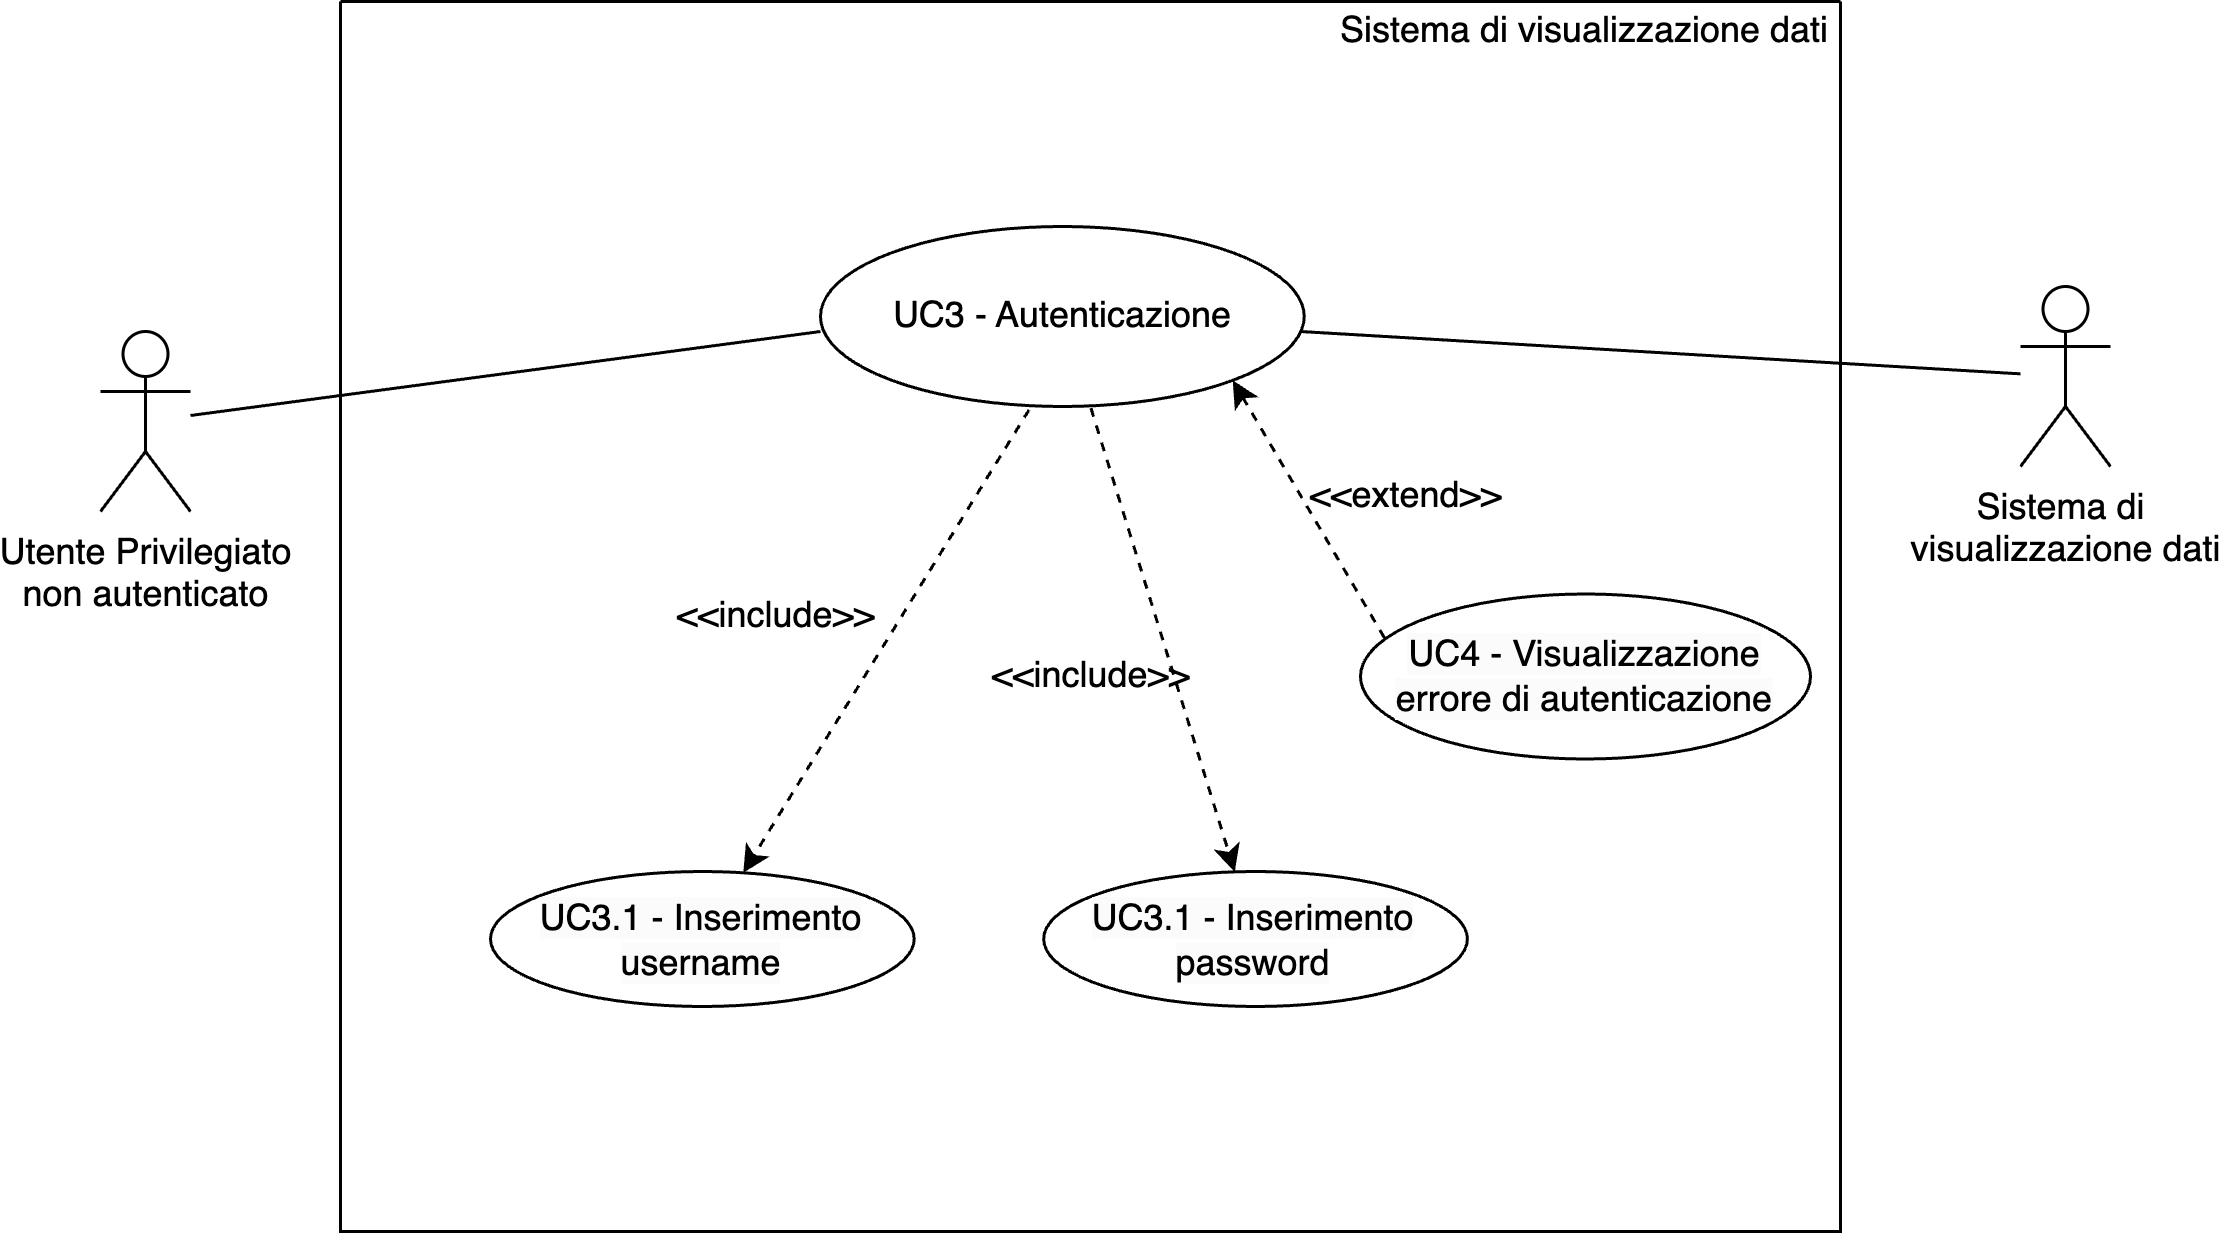
\includegraphics[width=0.7\linewidth]{UC3.12_UC4image.png}
    \caption{UC3 - Autenticazione\newline
    UC4 - Visualizzazione errore autenticazione}
    \label{fig:UC3 e UC4}
\end{figure}
%%%%%%%%%%%%%%%%%%%%%%%%%%%%%%%%%%%%%%%%%%%%%%%%%%%%%%%%%%%%%%%%%%%%%%%%%%%
\subsubsection{\textbf{UC3.1 - Inserimento username}}
\begin{itemize}
     \item \textbf{Attore$_G$ Principale:} Utente Privilegiato non autenticato.
     \item \textbf{Precondizioni:} 
            \begin{itemize}
                \item L'utente privilegiato non autenticato sta eseguendo l'autenticazione (UC3).
            \end{itemize}
     \item \textbf{Postcondizioni:} Il nome utente è stato inserito nel campo dati preposto.
     \item \textbf{Scenario Principale:}
        \begin{enumerate}
            \item L'utente privilegiato non autenticato inserisce il suo username nell'apposito campo dati.
        \end{enumerate}
     \item \textbf{User-Story$_G$ associata:} Come utente privilegiato non autenticato  voglio poter inserire lo username al fine di eseguire l'accesso.
\end{itemize}
%%%%%%%%%%%%%%%%%%%%%%%%%%%%%%%%%%%%%%%%%%%%%%%%%%%%%%%%%%%%%%%%%%%%%%%%%%%
\subsubsection{\textbf{UC3.2 - Inserimento password}}
\begin{itemize}
     \item \textbf{Attore$_G$ Principale:} Utente Privilegiato non autenticato.
     \item \textbf{Precondizioni:} 
        \begin{itemize}
            \item L'utente privilegiato non autenticato sta eseguendo l'autenticazione (UC3).
        \end{itemize}
     \item \textbf{Postcondizioni:} La password è stata inserita nel campo dati preposto.
     \item \textbf{Scenario Principale:}
        \begin{enumerate}
            \item L'utente privilegiato non autenticato inserisce la sua password nell'apposito campo dati.
        \end{enumerate}
     \item \textbf{User-Story$_G$ associata:} Come utente privilegiato non autenticato voglio poter inserire la password al fine di eseguire l'accesso.
\end{itemize}
%%%%%%%%%%%%%%%%%%%%%%%%%%%%%%%%%%%%%%%%%%%%%%%%%%%%%%%%%%%%%%%%%%%%%%%%%%%
\subsubsection{\textbf{UC4 - Visualizzazione errore autenticazione}}
\begin{itemize}
    \item \textbf{Attore$_G$ Principale:} Utente privilegiato non autenticato.
    \item \textbf{Precondizioni:}
        \begin{itemize}
            \item Il sistema è operativo e accessibile.
            \item L'utente privilegiato non autenticato ha inserito una combinazione non valida di username e password.
            \item L'autenticazione (UC3) è fallita.
        \end{itemize}
    \item \textbf{Postcondizioni:}
        \begin{itemize}
            \item L’utente privilegiato non autenticato visualizza un messaggio di errore.
            \item L’utente privilegiato non autenticato può correggere le credenziali e provare ad effettuare nuovamente l'autenticazione.
        \end{itemize}
    \item \textbf{Scenario Principale:}
        \begin{enumerate}
            \item L'utente privilegiato non autenticato inserisce le credenziali e effettua l'accesso.
            \item Il sistema verifica le credenziali inserite e se una delle due o entrambe non sono valide fa visualizzare un messaggio di errore.
        \end{enumerate}
    \item \textbf{User-Story$_G$ associata:} Come utente privilegiato non autenticato, voglio poter visualizzare un messaggio di errore nel caso avessi inserito le credenziali errate.
\end{itemize}
%%%%%%%%%%%%%%%%%%%%%%%%%%%%%%%%%%%%%%%%%%%%%%%%%%%%%%%%%%%%%%%%%%%%%%%%%%%
\subsubsection{\textbf{UC1 - Visualizzazione Dashboard$_G$}}
\begin{figure}[H]
    \centering
    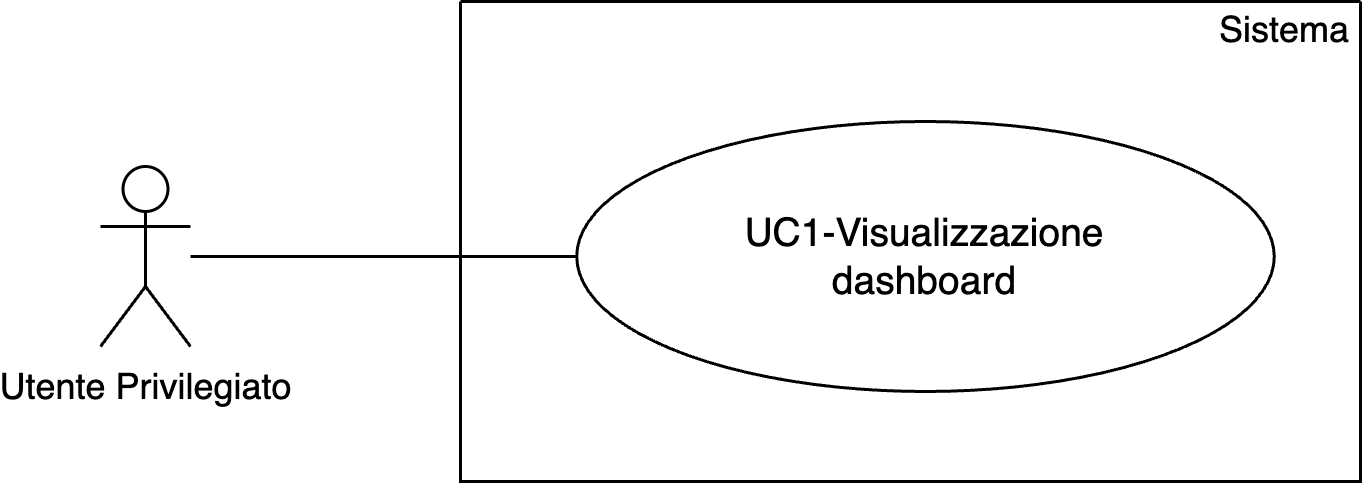
\includegraphics[width=0.7\linewidth]{UC1image.png}
    \caption{UC1 - Visualizzazione Dashboard$_G$}
    \label{fig:UC1}
\end{figure}
\begin{itemize}
    \item \textbf{Attore$_G$ Principale:} Utente privilegiato.
    \item \textbf{Precondizioni:} 
        \begin{itemize}
          \item Il sistema è operativo e accessibile;
            \item L'utente privilegiato ha effettuato l'accesso (UC3).
        \end{itemize}
    \item \textbf{Postcondizioni:} L'utente privilegiato è in grado di visualizzare una mappa geografica, con i sensori GPS aggiornati in tempo reale (percorsi degli utenti), i vari punti di interesse e le pubblicità offerte agli utenti.
    \item \textbf{Scenario Principale:}
        \begin{enumerate}
            \item L'utente privilegiato accede alla piattaforma di visualizzazione della Dashboard$_G$.
            \item Il sistema mette a disposizione tutte le informazioni storicizzate e ricevute dai sensori, distribuiti su una mappa tramite marker.
        \end{enumerate}
    \item \textbf{User-Story$_G$ associata:} Come utente privilegiato, voglio accedere alla Dashboard$_G$ per visualizzare in tempo reale i mezzi che ho messo a noleggio (sensori GPS), i punti di interesse che usufruiscono di questo servizio e le inserzioni che vengono generate per gli utenti che hanno effettuato il noleggio.
\end{itemize}

%%%%%%%%%%%%%%%%%%%%%%%%%%%%%%%%%%%%%%%%%%%%%%%%%%%%%%%%%%%%%%%%%%%%%%%%%%%

\subsubsection{\textbf{UC1.1 - Visualizzazione percorsi sulla mappa}}
\begin{figure}[H]
    \centering
    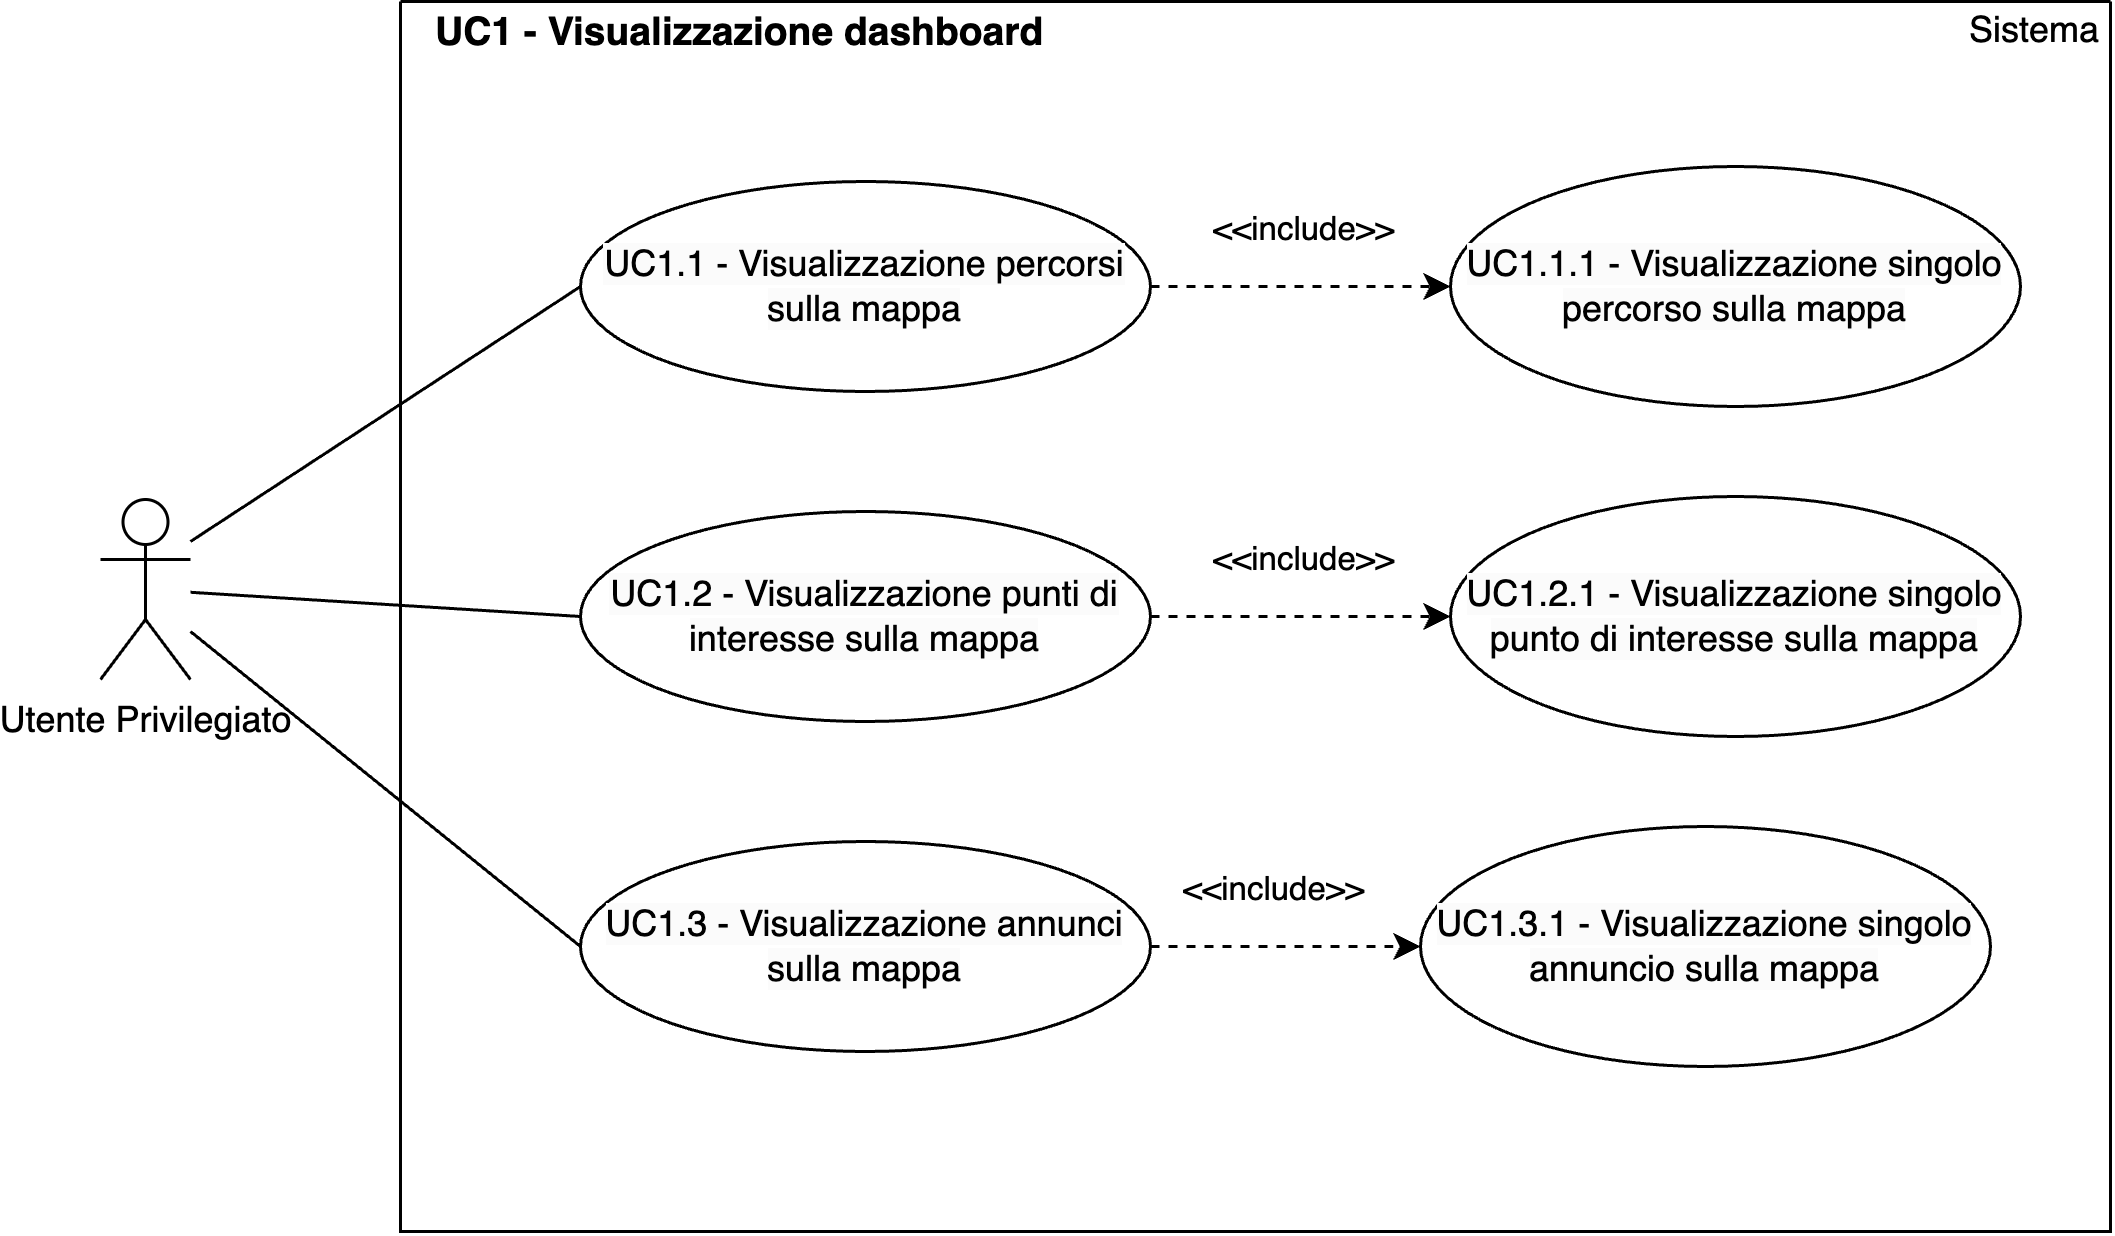
\includegraphics[width=0.7\linewidth]{UC1.123image.png}
    \caption{ UC1.1 - Visualizzazione percorsi sulla mappa -- UC1.2 - Visualizzazione punti di interesse sulla mappa -- UC1.3 - Visualizzazione annunci sulla mappa}
    \label{fig:UC1.1}
\end{figure}
\label{UC1.1}
\begin{itemize}
     \item \textbf{Attore$_G$ Principale:} Utente Privilegiato.
     \item \textbf{Precondizioni:}
        \begin{itemize}
    		\item L'utente privilegiato ha effettuato l'accesso e sta      visualizzando la Dashboard$_G$ (UC3 e UC1).
        \end{itemize}
     \item \textbf{Postcondizioni:} L'utente privilegiato è in grado di visualizzare i percorsi degli utenti differenziati dai marker presenti sulla mappa.
     \item \textbf{Scenario Principale:}
        \begin{enumerate}
            \item L'utente privilegiato ha accesso alla Dashboard$_G$ con la mappa interattiva (UC3 e UC1);
            \item L'utente privilegiato visualizza i percorsi di tutti gli utenti attivi nel sistema;
        \end{enumerate}
     \item \textbf{User-Story$_G$ associata:}
     Come utente privilegiato voglio poter visualizzare i vari percorsi effettuati dagli utenti. Questa Dashboard$_G$ permette di tenere traccia dei percorsi, tramite dei marker che rappresentano le più recenti posizioni GPS tracciate dal sistema.
\end{itemize}
%%%%%%%%%%%%%%%%%%%%%%%%%%%%%%%%%%%%%%%%%%%%%%%%%%%%%%%%%%%%%%%%%%%%%%%%%%%
\subsubsection{\textbf{UC1.2 - Visualizzazione punti di interesse sulla mappa}}
\label{UC1.2}
\begin{itemize}
     \item \textbf{Attore$_G$ Principale:} Utente Privilegiato.
     \item \textbf{Precondizioni:}
        \begin{itemize}
    		\item L'utente privilegiato ha effettuato l'accesso e sta visualizzando la Dashboard$_G$ principale (UC3 e UC1) o la Dashboard$_G$ singolo utente(UC1.1.1).
        \end{itemize}
     \item \textbf{Postcondizioni:} L'utente privilegiato è in grado di visualizzare tutti i punti di interesse riconosciuti dal sistema tramite dei marker sulla mappa.
     \item \textbf{Scenario Principale:}
        \begin{enumerate}
            \item L'utente privilegiato ha accesso alla Dashboard$_G$ con la mappa interattiva (UC3 e UC1)
            \item Il sistema mette a disposizione tutti i punti di interesse attivi in quel momento.
        \end{enumerate}
     \item \textbf{User-Story$_G$ associata:}
     Come utente privilegiato voglio poter visualizzare tutti i punti di interesse presenti sulla mappa.
\end{itemize}
%%%%%%%%%%%%%%%%%%%%%%%%%%%%%%%%%%%%%%%%%%%%%%%%%%%%%%%%%%%%%%%%%%%%%%%%%%%
\subsubsection{\textbf{UC1.3 - Visualizzazione annunci sulla mappa}}
\label{UC1.3}
\begin{itemize}
    \item \textbf{Attore$_G$ Principale:} Utente privilegiato.
    \item \textbf{Precondizioni:} 
        \begin{itemize}
         \item Il sistema è operativo e accessibile.
    	\item L'utente privilegiato ha effettuato l'accesso e sta          visualizzando la Dashboard$_G$ principale (UC3 e UC1) o la Dashboard$_G$ singolo utente(UC1.1.1).
        \end{itemize}
    \item \textbf{Postcondizioni:} L'Utente privilegiato visualizzerà un marker che rappresenta un annuncio personalizzato del punto di interesse in base ai dati dell'utente che passa vicino a quel punto. 
    \item \textbf{Scenario Principale:} 
        \begin{enumerate}
    	\item Un utente, mentre si muove sulla mappa, passa nell'area      di un punto di interesse.
    	\item Il sistema elabora le informazioni dell'utente e del         punto di interesse per generare il testo dell'eventuale            annuncio;
        \item Il sistema fa visualizzare un marker sulla mappa, che rappresenta l'annuncio generato.
	\end{enumerate}
    \item \textbf{User-Story$_G$ associata:} Come utente privilegiato voglio visualizzare sulla mappa gli annunci pubblicitari che arrivano ai vari utenti.
\end{itemize}
%%%%%%%%%%%%%%%%%%%%%%%%%%%%%%%%%%%%%%%%%%%%%%%%%%%%%%%%%%%%%%%%%%%%%%%%%%%
\subsubsection{\textbf{UC1.1.1 - Visualizzazione mappa singolo utente}}
\begin{figure}[H]
    \centering
    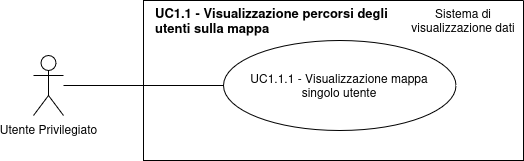
\includegraphics[width=0.7\linewidth]{UC1.1.1image.png}
    \caption{UC1.1.1 - Visualizzazione mappa singolo utente}
    \label{fig:UC1.1.1}
\end{figure}
\label{UC1.1.1}
\begin{itemize}
     \item \textbf{Attore$_G$ Principale:} Utente Privilegiato.
     \item \textbf{Precondizioni:}
        \begin{itemize}
    		\item L'utente privilegiato ha effettuato l'accesso e sta      visualizzando la Dashboard$_G$ (UC3 e UC1).
    	        \item L'utente privilegiato ha selezionato un marker  presente sulla mappa dei percorsi(UC1.1).
        \end{itemize}
     \item \textbf{Postcondizioni:} L'utente privilegiato è in grado di ottenere informazioni più dettagliate del marker selezionato tramite una Dashboard$_G$ apposita.
     \item \textbf{Scenario Principale:}
        \begin{enumerate}
            \item L'utente privilegiato ha accesso alla Dashboard$_G$ con la mappa interattiva (UC3 e UC1);
            \item L'utente privilegiato seleziona un marker di un determinato percorso per visualizzarne la Dashboard$_G$ specifica;
            \item Il sistema mette a disposizione lo storico delle posizioni e dei messaggi archiviati per quel marker.
        \end{enumerate}
     \item \textbf{User-Story$_G$ associata:}
     Come utente privilegiato voglio selezionare i vari marker, che indicano i mezzi di trasporto, presenti sulla mappa dei percorsi, in modo da visualizzare una Dashboard$_G$ contenente le informazioni relative ad un singolo utente. Questa Dashboard$_G$ permette di visualizzare i dettagli sullo storico completo delle posizioni e sull'utente che sta utilizzando il mezzo. Inoltre permette di poter vedere tutti gli annunci inviati a quell'utente durante la stessa giornata.
\end{itemize}

%%%%%%%%%%%%%%%%%%%%%%%%%%%%%%%%%%%%%%%%%%%%%%%%%%%%%%%%%%%%%%%%%%%%%%%%%%%
\subsubsection{\textbf{UC1.1.1.1 - Visualizzazione dettagli dei marker utente sulla mappa}}
\begin{figure}[H]
    \centering
    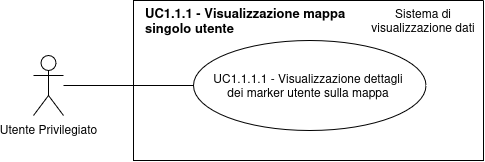
\includegraphics[width=0.7\linewidth]{UC1.1.1.1image.png}
    \caption{UC1.1.1.1 - Visualizzazione dettagli dei marker utente sulla mappa}
    \label{fig:UC1.1.1.1}
\end{figure}
\label{UC1.1.1.1}
\begin{itemize}
     \item \textbf{Attore$_G$ Principale:} Utente Privilegiato.
     \item \textbf{Precondizioni:}
        \begin{itemize}
        \item L'utente privilegiato ha selezionato un marker, raffigurante un percorso di un singolo utente, e sta visualizzando la Dashboard$_G$ di singolo utente (UC1.1.1);
          \item L'utente privilegiato ha selezionato un marker utente presente nella mappa di singolo utente.
        \end{itemize}
      \item \textbf{Postcondizioni:} L'utente privilegiato visualizza un pannello contenente le informazioni del marker utente selezionato in forma tabellare. La tabella conterrà la posizione, espressa in latitudine e longitudine,l'istante di rilevamento e i dati dell'utente che sta utilizzando il mezzo. I dati dell'utente presenti in tabella saranno:
        \begin{itemize}
        \item Nome;
        \item Cognome;
        \item Email;
        \item Genere;
        \item Data di nascita;
        \item Stato civile.
        \end{itemize}
      \item \textbf{Scenario Principale:}
        \begin{enumerate}
            \item L'utente privilegiato ha accesso alla Dashboard$_G$ di un singolo utente(UC1.1.1);
            \item L'utente privilegiato seleziona un marker utente presente sulla mappa di un singolo utente;
            \item Il sistema riporta le informazioni del marker in forma tabellare.
        \end{enumerate}
     \item \textbf{User-Story$_G$ associata:}
       Come utente privilegiato voglio selezionare i marker, che indicano le posizioni di un singolo utente, presenti sulla mappa di singolo utente, per poter visualizzare le informazioni specifiche di ogni istante.
\end{itemize}

%%%%%%%%%%%%%%%%%%%%%%%%%%%%%%%%%%%%%%%%%%%%%%%%%%%%%%%%%%%%%%%%%%%%%%%%%%%
%%%%%%%%%%%%%%%%%%%%%%%%%%%%%%%%%%%%%%%%%%%%%%%%%%%%%%%%%%%%%%%%%%%%%%%%%%%
\subsubsection{\textbf{UC1.2.1 - Visualizzazione area del punto di interesse}}
\begin{figure}[H]
    \centering
    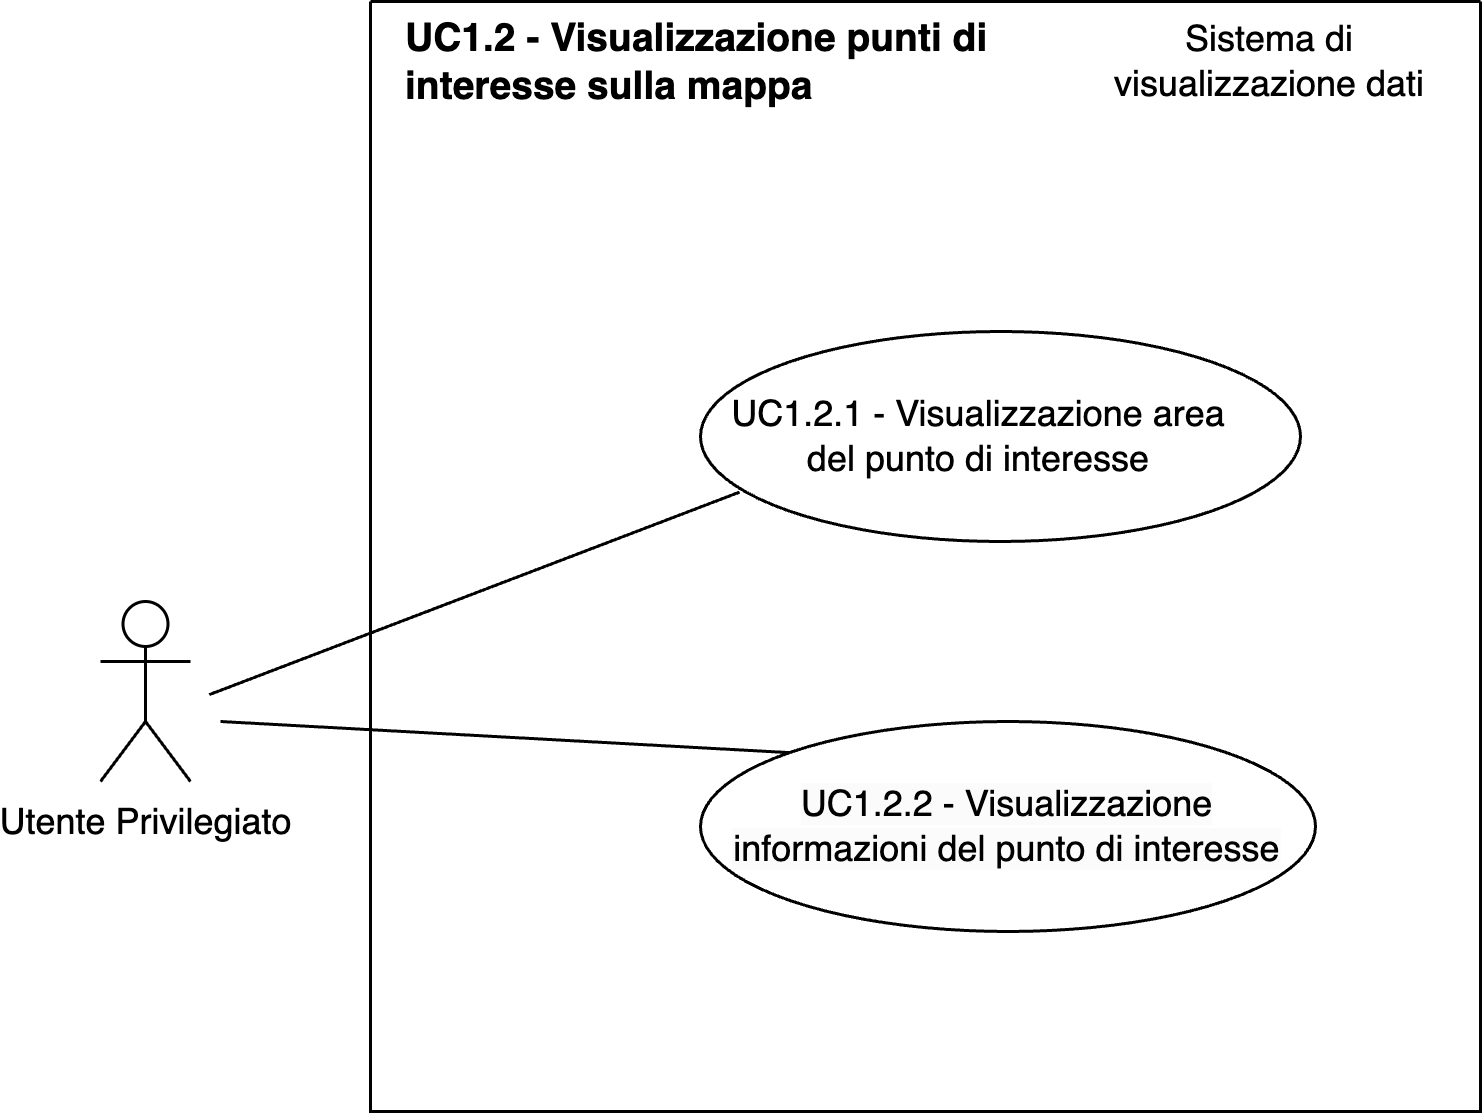
\includegraphics[width=0.7\linewidth]{UC1.2.12image.png}
    \caption{UC1.2.1 - Visualizzazione area del punto di interesse -- UC1.2.2 - Visualizzazione informazioni del punto di interesse}
    \label{fig:UC1.2.1-UC1.2.2}
\end{figure}
\begin{itemize}
     \item \textbf{Attore$_G$ Principale:} Utente Privilegiato.
     \item \textbf{Precondizioni:}
        \begin{itemize}
            \item L'utente privilegiato ha selezionato un punto di interesse (UC1.2).
        \end{itemize}
     \item \textbf{Postcondizioni:} L'utente privilegiato è in grado di visualizzare l'area di influenza di un punto di interesse visibile sulla mappa.
     \item \textbf{Scenario Principale:}
        \begin{enumerate}
            \item Il sistema genera l'area di influenza del punto di interesse selezionato e la mostra sulla mappa.
        \end{enumerate}
     \item \textbf{User-Story$_G$ associata:}
     Come utente privilegiato voglio vedere l'area di influenza di ogni punto di interesse presente sulla mappa.
\end{itemize}

%%%%%%%%%%%%%%%%%%%%%%%%%%%%%%%%%%%%%%%%%%%%%%%%%%%%%%%%%%%%%%%%%%%%%%%%%%%
 \subsubsection{\textbf{UC1.2.2 - Visualizzazione informazioni del punto di interesse}}
 \label{UC1.2.2}
 \begin{itemize}
     \item \textbf{Attore$_G$ Principale:} Utente Privilegiato
     \item \textbf{Precondizioni:}
       \begin{itemize}
            \item L'utente privilegiato ha effettuato l'accesso e sta visualizzando la Dashboard$_G$ (UC3 e UC1).
            \item L'utente privilegiato ha selezionato un punto di interesse (UC1.2).
       \end{itemize}
     \item \textbf{Postcondizioni:} L'utente privilegiato visualizza un pannello contenente una tabella, che esprime le informazioni specifiche del punto di interesse selezionato. Tali informazioni sono:
       \begin{itemize}
       \item il nome;
       \item la posizione espressa in latitudine e longitudine;
       \item l'indirizzo;
       \item la tipologia, cioè di che ambito si occupa il punto di interesse;
       \item la descrizione.
       \end{itemize}
     \item \textbf{Scenario Principale:}
        \begin{enumerate}
          \item L'utente privilegiato ha selezionato un punto di interesse presente sulla mappa;
            \item Il sistema riporta le informazioni del punto di interesse selezionato e le mostra nella Dashboard$_G$ in forma tabellare.
        \end{enumerate}
     \item \textbf{User-Story$_G$ associata:} Come utente privilegiato voglio visualizzare le informazioni di un punto di interesse presente sulla mappa. 
 \end{itemize}


%%%%%%%%%%%%%%%%%%%%%%%%%%%%%%%%%%%%%%%%%%%%%%%%%%%%%%%%%%%%%%%%%%%%%%%%%%%

\subsubsection{\textbf{UC1.3.1 - Visualizzazione informazioni dell'annuncio}}
\begin{figure}[H]
    \centering
    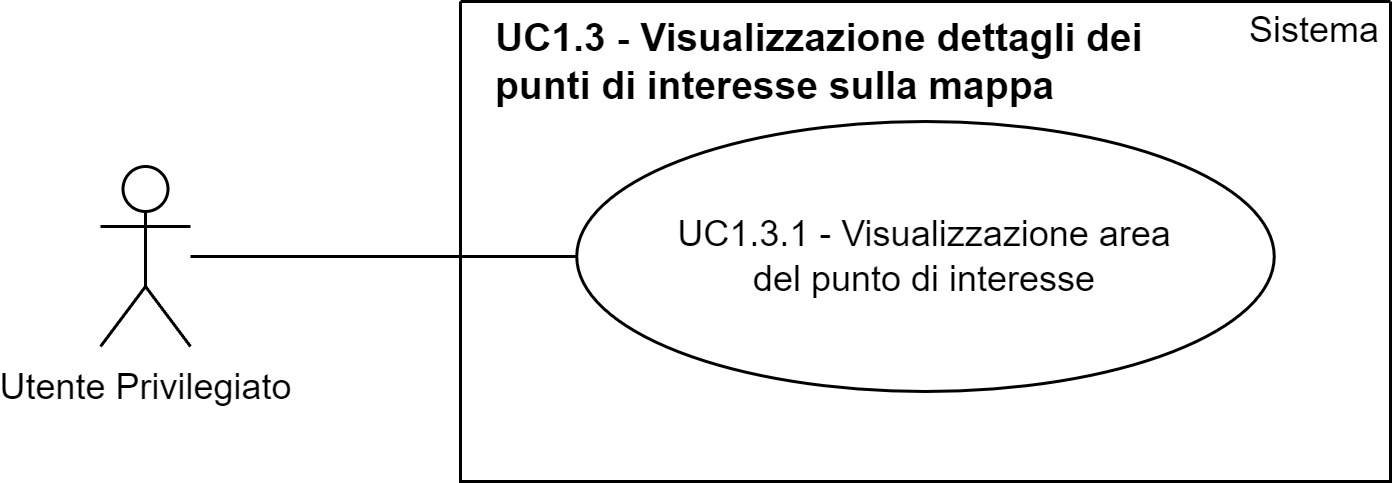
\includegraphics[width=0.7\linewidth]{UC1.3.1image.png}
    \caption{UC1.3.1 - Visualizzazione informazioni dell'annuncio}
    \label{fig:UC1.3.1}
\end{figure}
\label{UC1.3.1}
\begin{itemize}
    \item \textbf{Attore$_G$ Principale:} Utente privilegiato.
    \item \textbf{Precondizioni:} 
        \begin{itemize}
          \item L'utente privilegiato sta visualizzando un annuncio sulla mappa (UC1.3);
    	\item L'utente privilegiato ha selezionato un annuncio comparso sulla mappa.
        \end{itemize}
    \item \textbf{Postcondizioni:} L'utente privilegiato visualizza un pannello contenente le informazioni dell'annuncio selezionato in forma tabellare. La tabella conterrà i nomi dell'utente e del punto di interesse coinvolti, la longitudine e latitudine di questi ultimi e il contenuto effettivo dell'annuncio.
    \item \textbf{Scenario Principale:} 
        \begin{enumerate}
          \item L'utente privilegiato ha selezionato un annuncio presente sulla mappa;
            \item Il sistema riporta le informazioni dell'annuncio selezionato e le mostra nella Dashboard$_G$ in forma tabellare.
	\end{enumerate}
    \item \textbf{User-Story$_G$ associata:} Come utente privilegiato voglio visualizzare le informazioni relative ad un annuncio pubblicitario creato.
\end{itemize}

%%%%%%%%%%%%%%%%%%%%%%%%%%%%%%%%%%%%%%%%%%%%%%%%%%%%%%%%%%%%%%%%%%%%%%%%%%%

%%%%%%%%%%%%%%%%%%%%%%%%%%%%%%%%%%%%%%%%%%%%%%%%%%%%%%%%%%%%%%%%%%%%%%%%%%%
\subsubsection{\textbf{UC2 - Visualizzazione annuncio}}
\begin{figure}[H]
    \centering
    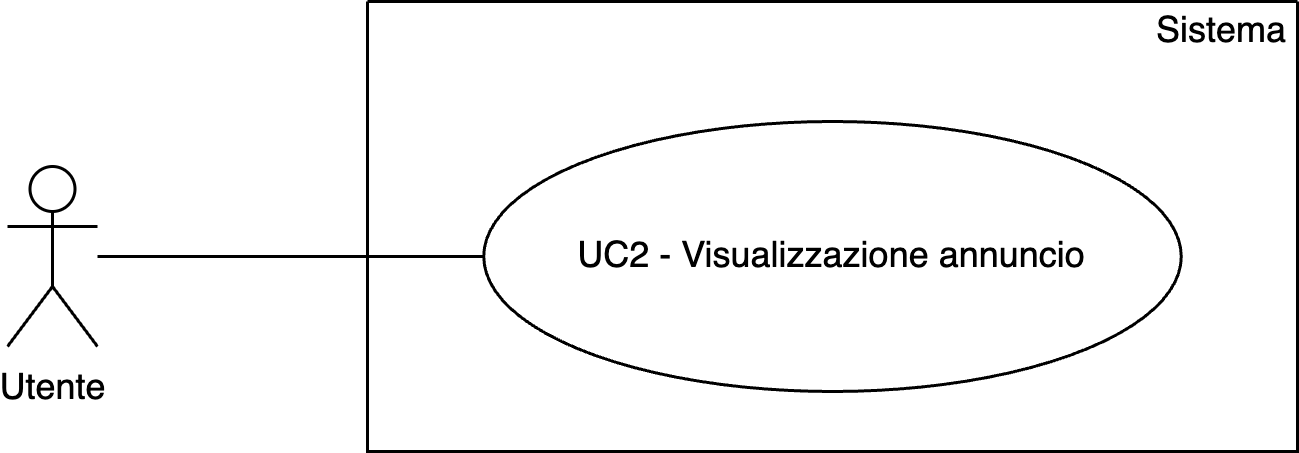
\includegraphics[width=0.7\linewidth]{UC2image.png}
    \caption{UC2 - Visualizzazione annuncio}
    \label{fig:UC2}
\end{figure}
\begin{itemize}
    \item \textbf{Attore$_G$ Principale:} Utente
    \item \textbf{Precondizioni:} 
        \begin{itemize}
    	\item Il sistema è operativo e accessibile.
    	\item Un utente entra nell'area di un punto di interesse.
        \end{itemize}
    \item \textbf{Postcondizioni:} L'Utente visualizzerà un messaggio contenente un annuncio personalizzato in base ai suoi dati personali e al punto di interesse.
    \item \textbf{Scenario Principale:} 
        \begin{enumerate}
            \item Un utente, mentre si muove sulla mappa, passa nell'area di un punto di interesse.
            \item Il sistema elabora le informazioni dell'utente e del punto di interesse per generare il testo dell'eventuale annuncio.
            \item Il sistema invia all'utente il messaggio contenente l'annuncio se questo è stato generato.
        \end{enumerate}
    \item \textbf{User-Story$_G$ associata:} Come utente voglio visualizzare gli annunci pubblicitari personalizzati che mi arrivano.
\end{itemize}
%%%%%%%%%%%%%%%%%%%%%%%%%%%%%%%%%%%%%%%%%%%%%%%%%%%%%%%%%%%%%%%%%%%%%%%%%%%
\subsubsection{\textbf{UC5 - Visualizzazione tabella dei PoI}}
\begin{figure}[H]
    \centering
    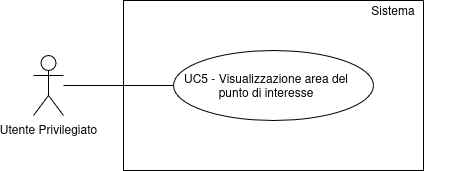
\includegraphics[width=0.7\linewidth]{UC5image.png}
    \caption{UC5 - Visualizzazione tabella dei PoI}
    \label{fig:UC5}
\end{figure}
\label{UC5}
\begin{itemize}
    \item \textbf{Attore$_G$ Principale:} Utente Privilegiato
    \item \textbf{Precondizioni:} 
        \begin{itemize}
          \item Il sistema è operativo e accessibile;
            \item L'utente privilegiato ha effettuato l'accesso (UC3).
        \end{itemize}
      \item \textbf{Postcondizioni:} L'utente è in grado di visualizzare una tabella contenenti i dati dei singoli PoI ordinati per la quantità di messaggi inviati in questo mese.\\
        Altre informazioni dei PoI presenti in tabella sono:
        \begin{itemize}
       \item il nome;
       \item l'indirizzo;
       \item la tipologia, cioè di che ambito si occupa il punto di interesse;
       \item la descrizione;
         \item numero di messaggi inviati durante il mese.
        \end{itemize}
    \item \textbf{Scenario Principale:} 
        \begin{enumerate}
        \item L'utente privilegiato accede alla piattaforma e seleziona la visualizzazione della tabella dei PoI;
          \item Il sistema mette a disposizioni le informazioni storicizzate per ogni singolo PoI in forma tabellare.
        \end{enumerate}
    \item \textbf{User-Story$_G$ associata:} Come utente privilegiato, voglio accedere alla tabella dei PoI per poter visualizzare quale PoI sta inviando più messaggi in quel mese e poter visionare facilmente le informazioni di ogni singolo PoI.
\end{itemize}

%%%%%%%%%%%%%%%%%%%%%%%%%%%%%%%%%%%%%%%%%%%%%%%%%%%%%%%%%%%%%%%%%%%%%%%%%%%
\subsubsection{\textbf{UC6 - Trasmissione dati geoposizionali}}
\begin{figure}[H]
    \centering
    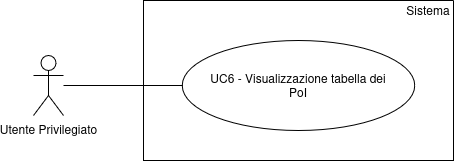
\includegraphics[width=0.7\linewidth]{UC6image.png}
    \caption{UC6 - Trasmissione dati geoposizionali}
    \label{fig:UC6}
\end{figure}
\label{UC6}
\begin{itemize}
    \item \textbf{Attore$_G$ Principale:} Sensore
    \item \textbf{Attore$_G$ Secondario:} Sistema di Stream Processing
    \item \textbf{Precondizioni:} 
        \begin{itemize}
    	\item Il sensore è attivo e connesso al sistema.
        \end{itemize}
    \item \textbf{Postcondizioni:} Il sensore invia i dati posizionali del mezzo al sistema di stream processing.
    \item \textbf{Scenario Principale:} 
        \begin{enumerate}
            \item Il sensore di tipo GPS effettua un rilevamento della posizione geografica dell'utente espressa in latitudine e longitudine;
            \item Il sensore GPS invia i dati posizionali al sistema di stream processing.
        \end{enumerate}
    \item \textbf{User-Story$_G$ associata:} Come Sensore GPS, desidero trasmettere la posizione espressa in latitudine e longitudine al sistema di stream processing.

\end{itemize}

%%%%%%%%%%%%%%%%%%%%%%%%%%%%%%%%%%%%%%%%%%%%%%%%%%%%%%%%%%%%%%%%%%%%%%%%%%%

\subsubsection{\textbf{UC7 - Filtraggio e parsing dei dati ricevuti}}
\begin{figure}[H]
    \centering
    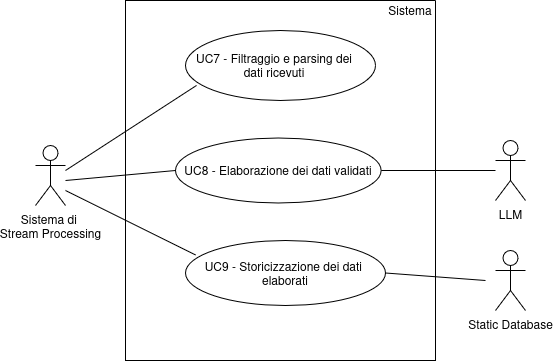
\includegraphics[width=0.7\linewidth]{UC789image.png}
    \caption{UC7 - Filtraggio e parsing dei dati ricevuti -- UC8 - Mapping dei dati validati -- UC9 - Storicizzazione dei dati elaborati}
    \label{fig:UC789}
\end{figure}
\label{UC7}
\begin{itemize}
    \item \textbf{Attore$_G$ Principale:} Sistema di Stream Processing
    \item \textbf{Precondizioni:} 
        \begin{itemize}
          \item Il sistema è operativo e accessibile;
            \item Il sistema di Stream Processing è attivo e sta ricevendo dati dai sensori (UC6).
        \end{itemize}
      \item \textbf{Postcondizioni:} 
        I dati ricevuti vengono filtrati per definire che siano validi ed infine viene effettuato un parsing per facilitarne l'elaborazione.\\
    \item \textbf{Scenario Principale:} 
        \begin{enumerate}
        \item Il sistema di stream processing è attivo e sta ricevendo dati posizionali espressi in latitudine e longitudine in ingresso dai sensori (UC6), id del mezzo e l'istante di invio dei dati dal sensore;
        \item Il sistema filtra i dati, in modo da scartare dati non validi o non consistenti;
        \item Il sistema fa un parsing dei dati, distinguendo i diversi tipi e campi dato.
        \end{enumerate}
    \item \textbf{User-Story$_G$ associata:} Come sistema di Stream Processing voglio poter filtrare i dati ricevuti in ingresso secondo le linee guida, per poi validare e interpretare la struttura (parsing)
\end{itemize}


%%%%%%%%%%%%%%%%%%%%%%%%%%%%%%%%%%%%%%%%%%%%%%%%%%%%%%%%%%%%%%%%%%%%%%%%%%%

\subsubsection{\textbf{UC8 - Elaborazione dei dati validati}}

\label{UC8}
\begin{itemize}
    \item \textbf{Attore$_G$ Principale:} Sistema di Stream Processing
    \item \textbf{Attore$_G$ Secondario:} LLM
    \item \textbf{Precondizioni:} 
        \begin{itemize}
          \item Il sistema è operativo e accessibile;
            \item Il sistema di Stream Processing è attivo e ha validato i dati che costantemente riceve in input (UC7).
        \end{itemize}
      \item \textbf{Postcondizioni:} I dati ricevuti vengono elaborati tramite richiesta ad un LLM, che fornirà la risposta valida per il sistema\\
    \item \textbf{Scenario Principale:} 
        \begin{enumerate}
        \item Il sistema di stream processing è attivo e sta ricevendo i dati posizionali (latitudine e longitudine), id del mezzo e l'istante di rilevamento;
        \item Il sistema ha filtrato ed effettuato il parsing dei dati (UC7);
        \item Il sistema fa un'elaborazione dei dati tramite richiesta ad un LLM.
        \end{enumerate}
    \item \textbf{User-Story$_G$ associata:} Come sistema di Stream Processing voglio poter elaborare i dati validati. Per fare ciò richiedo che parte dell'elaborazione sia effettuata da un sistema esterno di LLM per ottenere una risposta rilevante per il mio sistema.
\end{itemize}

%%%%%%%%%%%%%%%%%%%%%%%%%%%%%%%%%%%%%%%%%%%%%%%%%%%%%%%%%%%%%%%%%%%%%%%%%%%

\subsubsection{\textbf{UC9 - Storicizzazione dei dati elaborati}}

\label{UC9}
\begin{itemize}
    \item \textbf{Attore$_G$ Principale:} Sistema di Stream Processing
    \item \textbf{Attore$_G$ Secondario:} Database
    \item \textbf{Precondizioni:} 
        \begin{itemize}
          \item Il sistema è operativo e accessibile;
            \item Il sistema di Stream Processing è attivo e ha elaborato i dati ricevuti in input (UC8).
        \end{itemize}
      \item \textbf{Postcondizioni:} I dati elaborati dal sistema di Stream Processing, vengono storicizzati in un database per garantirne la trasparenza e integrità.\\
    \item \textbf{Scenario Principale:} 
        \begin{enumerate}
        \item Il sistema di stream processing è attivo e sta ricevendo dati in ingresso;
        \item Il sistema ha filtrato ed effettuato l'elaborazione dei dati;
        \item Il sistema serializza i dati posizionali (latitudine e longitudine), id del mezzo e l'istante di rilevamento in un database. 
        \end{enumerate}
    \item \textbf{User-Story$_G$ associata:} Come sistema di Stream Processing voglio poter storicizzare i dati validati ed elaborati, affinchè siano facilemente recuperabili o per effettuarne delle analisi in futuro.
\end{itemize}

%%%%%%%%%%%%%%%%%%%%%%%%%%%%%%%%%%%%%%%%%%%%%%%%%%%%%%%%%%%%%%%%%%%%%%%%%%%

\subsubsection{\textbf{UC10 - Selezione del PoI più adeguato per l'utente}}
\begin{figure}[H]
    \centering
    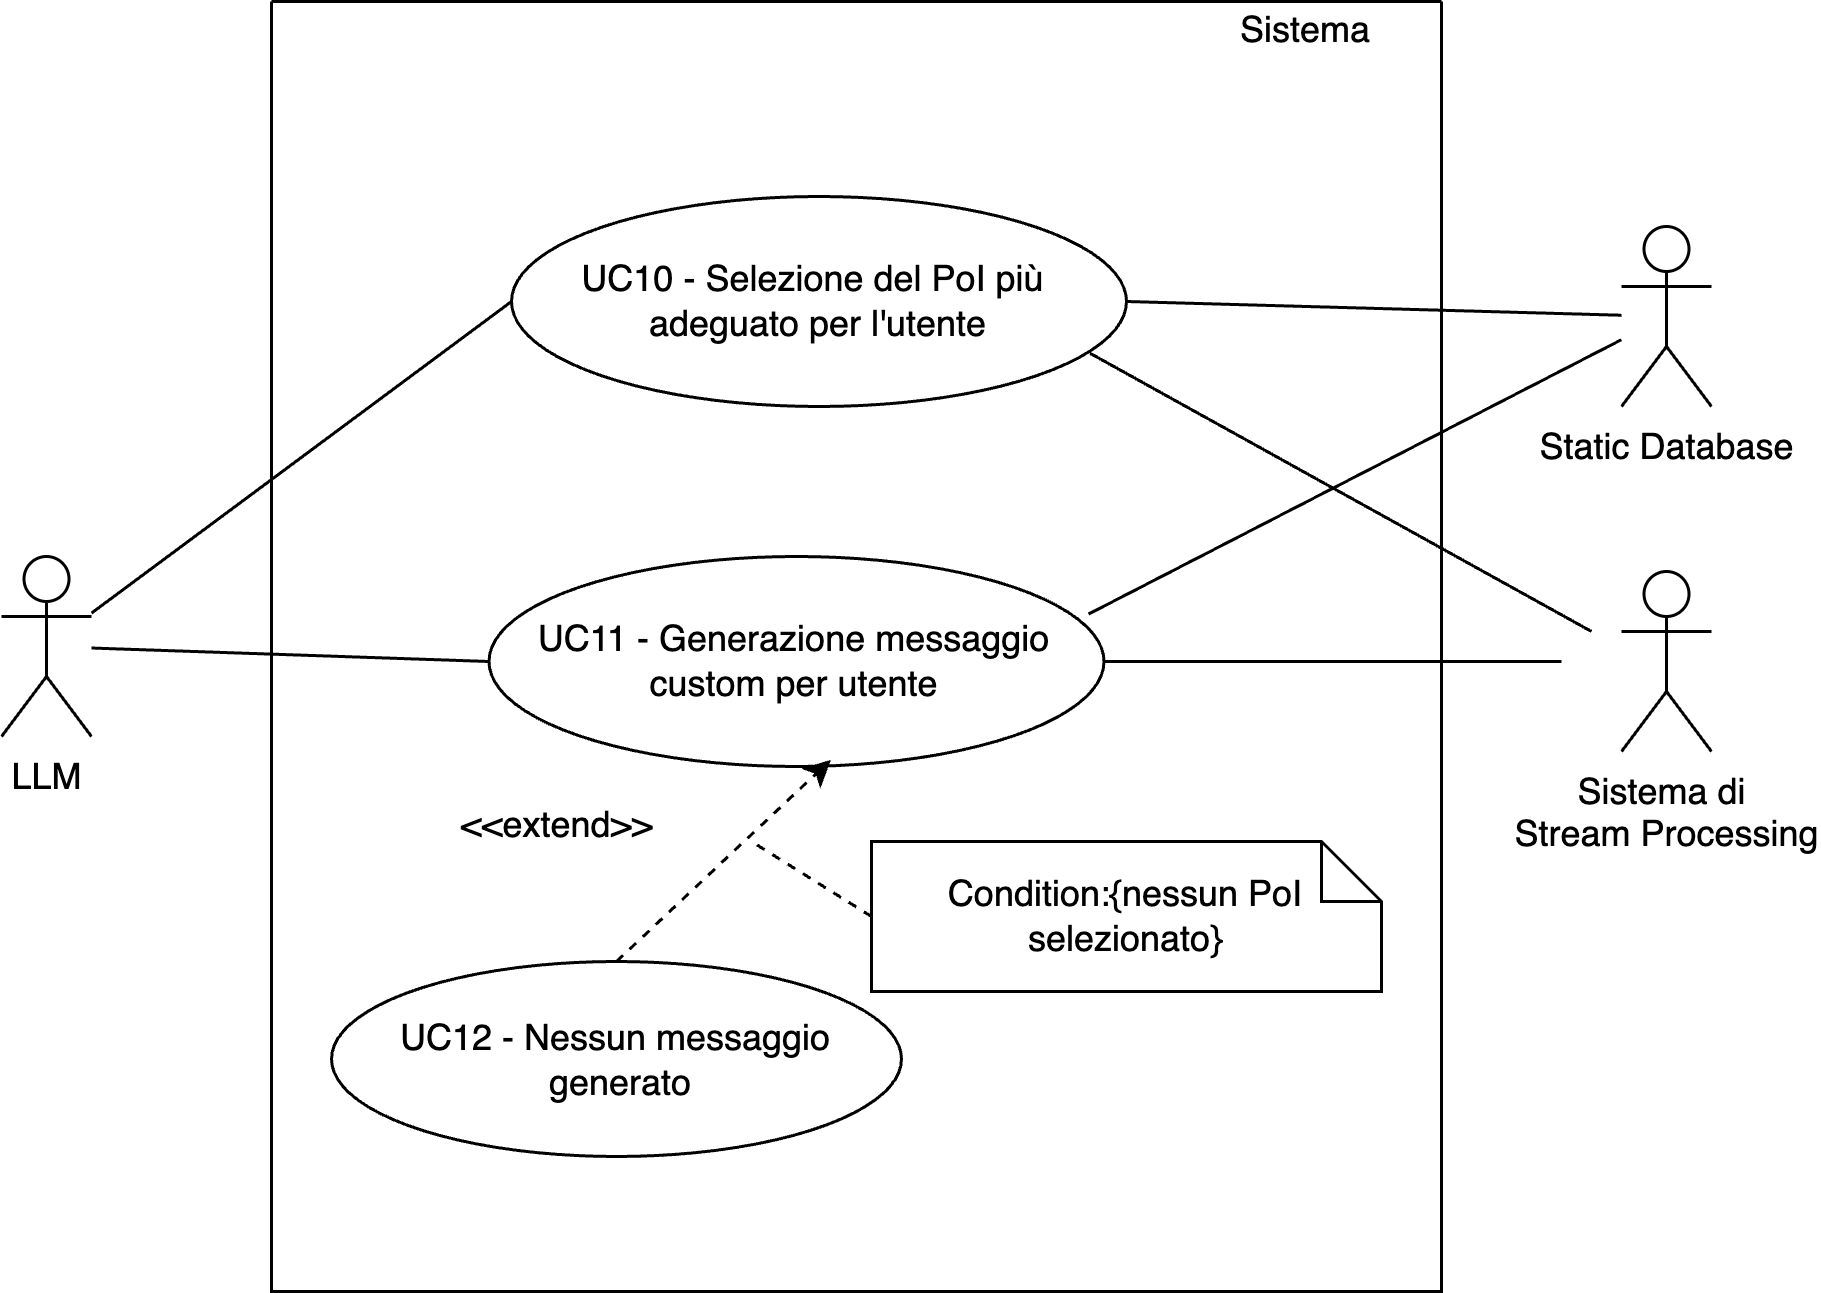
\includegraphics[width=0.7\linewidth]{UC101112image.png}
    \caption{UC10 - Selezione del PoI più adeguato per l'utente -- UC11 - Generazione messaggio custom per utente -- UC12 - Nessun messaggio generato}
    \label{fig:UC101112}
\end{figure}
\label{UC10}
\begin{itemize}
    \item \textbf{Attore$_G$ Principale:} LLM
    \item \textbf{Attori$_G$ Secondari:} 
    \begin{itemize}
        \item Database
        \item Sistema di Stream Processing
    \end{itemize}
    \item \textbf{Precondizioni:} 
        \begin{itemize}
          \item Il sistema è operativo e accessibile;
            \item Il database è aggiornato con i dati personali dell'utente e i suoi eventuali interessi;
            \item Il database è aggiornato con i dati dei punti di interesse rilevanti per l'utente in quell'istante;
            \item Il sistema di Stream Processing fornisce la posizione dell'utente in tempo reale dopo una validazione e parsing (UC7-8).
        \end{itemize}
      \item \textbf{Postcondizioni:} L'obiettivo è selezionare il punto di interesse (POI) più rilevante secondo gli interessi dell'utente. Il modello LLM utilizza le informazioni dei punti di interesse (Tipologia) e dell'utente (Interessi) presenti all'interno del Database per fare una selezione tra i punti di interesse proposti.\\
    \item \textbf{Scenario Principale:} 
        \begin{enumerate}
        \item L' LLM riceve i dati personali dell'utente:
          \begin{itemize}
          \item Nome;
          \item Cognome;
          \item Email;
          \item Genere;
          \item Data di nascita;
          \item Stato civile;
          \item Elenco di interessi dell'utente.
          \end{itemize}
          e quelli dei punti di interesse presenti nelle vicinanze dell'utente:
          \begin{itemize}
          \item Nome;
          \item Posizione espressa in latitudine e longitudine;
          \item Indirizzo;
          \item Tipologia, cioè di che ambito si occupa il punto di interesse;
          \item Descrizione.
          \end{itemize}
        \item L' LLM utilizza questi dati per filtrare i POI ricevuti sulla base degli interessi e profilazione utente;
        \item L' LLM ritorna il PoI più pertinente. 
        \end{enumerate}
    \item \textbf{User-Story$_G$ associata:} Come LLM voglio identificare e selezionare il Punto di Interesse più rilevante per l'utente in base alla sua profilazione e alle sue preferenze.
\end{itemize}

%%%%%%%%%%%%%%%%%%%%%%%%%%%%%%%%%%%%%%%%%%%%%%%%%%%%%%%%%%%%%%%%%%%%%%%%%%%

\subsubsection{\textbf{UC11 - Generazione messaggio custom per utente}}

\label{UC11}
\begin{itemize}
    \item \textbf{Attore$_G$ Principale:} LLM
    \item \textbf{Attori$_G$ Secondari:} 
    \begin{itemize}
        \item Database
        \item Sistema di Stream Processing
    \end{itemize}
    \item \textbf{Precondizioni:} 
        \begin{itemize}
          \item Il sistema è operativo e accessibile;
          \item Il database è aggiornato con i dati degli utenti registrati nel sistema;
            \item Il servizio di LLM ha identificato e serializzato in locale il punto di interesse più adeguato per l'utente (UC10).
        \end{itemize}
      \item \textbf{Postcondizioni:} Lo scopo è generare un annuncio personalizzato testuale da proporre all'utente durante il suo percorso con il mezzo di trasporto. Questo messaggio tiene conto della selezione del punto di interesse (PoI) (UC10) più rilevante alla profilazione del singolo utente (presente nel database). Infine il dato deve essere storicizzato nel database e inviato in un altra partizione del sistema di stream processing .\\
    \item \textbf{Scenario Principale:} 
        \begin{enumerate}
        \item L' LLM ha selezionato il punto di interesse più adeguato per l'utente in base alla posizione in tempo reale e il profilo (UC10);
        \item L' LLM utilizza le informazioni del PoI (nome, indirizzo, tipologia e descrizione) e del profilo utente (nome, cognome, genere, data di nascita e stato civile) per generare un annuncio testuale personalizzato;
        \item L' LLM invia al Sistema di Stream Processing il messaggio che verrà poi storicizzato nel Database e inviato all'utente.
        \end{enumerate}
    \item \textbf{Estensioni: } 
    \begin{itemize}
        \item UC12 - Nessun messaggio generato
    \end{itemize}
    \item \textbf{User-Story$_G$ associata:} Come LLM voglio generare un messaggio custom per l'utente basato sulla sua profilazione e su un PoI adeguato nel raggio della sua posizione in tempo reale.
\end{itemize}

%%%%%%%%%%%%%%%%%%%%%%%%%%%%%%%%%%%%%%%%%%%%%%%%%%%%%%%%%%%%%%%%%%%%%%%%%%%

\subsubsection{\textbf{UC12 - Nessun messaggio generato}}

\label{UC12}
\begin{itemize}
    \item \textbf{Attore$_G$ Principale:} LLM
    \item \textbf{Attori$_G$ Secondari:} 
    \begin{itemize}
        \item Database
        \item Sistema di Stream Processing
    \end{itemize}
    \item \textbf{Precondizioni:} 
        \begin{itemize}
          \item Il sistema è operativo e accessibile;
          \item Il database è aggiornato con i dati degli utenti registrati nel sistema;
          \item Il servizio di LLM non ha identificato il punto di interesse più adeguato per l'utente (condition).
        \end{itemize}
      \item \textbf{Postcondizioni:} Nessun messaggio personalizzato per l'utente viene generato durante l'elaborazione dell'ultima posizione inviata al sistema di Stream Processsing.\\
    \item \textbf{Scenario Principale:} 
        \begin{enumerate}
        \item L' LLM non ha selezionato il punto di interesse più adeguato per l'utente in base alla posizione in tempo reale e il profilo;
        \item L' LLM omette, per l'ultima rilevazione GPS, la generazione di un messaggio pubblicitario per l'utente.
        \end{enumerate}
    \item \textbf{User-Story$_G$ associata:} Come LLM voglio evitare di effettuare una richiesta al modello di AI, nel caso nessun punto di interesse sia stato selezionato per questa rilevazione GPS.
\end{itemize}

%%%%%%%%%%%%%%%%%%%%%%%%%%%%%%%%%%%%%%%%%%%%%%%%%%%%%%%%%%%%%%%%%%%%%%%%%%%


\newpage
\section{Requisiti$_G$}
%sicuramente da suddividere intenamente tra obbligatori, desiderabilli e opzionali

\subsection{Requisiti$_G$ funzionali}

% Definisci una nuova colonna centrata con larghezza fissa
\newcolumntype{C}[1]{>{\centering\arraybackslash}m{#1}}

\begin{center}
\renewcommand{\arraystretch}{1.5}
\begin{longtable}
{|>{\centering\arraybackslash}m{2.7cm}|>{\centering\arraybackslash}m{2.7cm}|>{\centering\arraybackslash}m{6cm}|>{\centering\arraybackslash}m{2.1cm}|}
%\begin{tabular}{|>{\vspace{5pt}}C{2.7cm}<{\vspace{5pt}}|>{\vspace{5pt}}C{2.7cm}<{\vspace{5pt}}|>{\vspace{5pt}}m{6cm}<{\vspace{5pt}}|>{\vspace{5pt}}C{2.1cm}<{\vspace{5pt}}|}
\hline
\textbf{Id. Requisito$_G$} & \textbf{Importanza} & \textbf{Descrizione} & \textbf{Fonti}\\
\endhead

\hline
 RF01 &  Obbligatorio &  L'utente privilegiato deve poter visualizzare la Dashboard$_G$ composta da una mappa interattiva con i vari marker su di essa. &  Capitolato$_G$, UC1\\
\hline
RF02 & Obbligatorio & L'utente privilegiato deve poter visualizzare dei marker che rappresentano i vari percorsi effettuati in tempo reale dagli utenti presenti nel sistema & Interna, UC1.1\\
\hline
RF03 & Obbligatorio & L'utente privilegiato deve poter visualizzare una Dashboard$_G$ relativa ad un singolo utente quando seleziona un marker. & Interna, UC1.1.1\\
\hline
RF04 & Obbligatorio & L'utente privilegiato deve poter visualizzare i dettagli del marker riguardante una singola posizione di un utente nella rispettiva dashboard & Interna, UC1.1.1.1\\
\hline
RF05 & Obbligatorio & L'utente privilegiato deve poter visualizzare tutti i punti di interesse riconosciuti dal sistema. & Interna, UC1.2\\
\hline
RF06 & Opzionale & L'utente privilegiato deve poter visualizzare l'area di influenza di un punto di interesse selezionato. & Interna, UC1.2.1\\
\hline
RF07 & Obbligatorio & L'utente privilegiato deve poter visualizzare le informazioni dettagliate di un punto di interesse quando selezionato. & Interna, UC1.2.2\\
\hline
RF08 & Obbligatorio & L'utente privilegiato deve poter visualizzare gli annunci pubblicitari provenienti da un determinato punto di interesse. & Capitolato$_G$, UC1.3\\
\hline
RF09 & Obbligatorio & L'utente privilegiato deve poter visualizzare i dettagli dell'annuncio generato & Interna, UC1.3.1\\
\hline
RF10 & Opzionale & L'utente deve poter visualizzare l'annuncio pubblicitario proveniente dal punto di interesse situato nell'area che sta attraversando. & Capitolato$_G$, UC2\\
\hline
RF11 & Obbligatorio & L'utente privilegiato deve poter effettuare l'accesso per visualizzare la Dashboard$_G$. & Capitolato$_G$, UC3, UC3.1, UC3.2\\
\hline
RF12 & Obbligatorio & L'utente privilegiato deve poter visualizzare un messaggio di errore nel caso le credenziali inserite durante l'accesso non siano riconosciute. & Capitolato$_G$, UC4\\
\hline
RF13 & Obbligatorio & L'utente privilegiato deve poter visualizzare una tabella contenente le informazioni dei singoli PoI e la quantità di messaggi inviati nel mese. & Interna, UC5\\
\hline
RF14 & Obbligatorio & Il sensore deve essere in grado di trasmettere i dati rilevati in tempo reale al sistema di Stream Processing. & Capitolato$_G$, UC6\\
\hline
RF15 & Obbligatorio & I dati ricevuti dal sensore devono essere filtrati e validati dal sistema di Stream Processing. & Interna, UC7\\
\hline
RF16 & Obbligatorio & I dati validati dal sistema di Stream Processing devono essere elaborati tramite un servizio LLM & Capitolato, UC8\\
\hline
RF17 & Obbligatorio & I dati elaborati dal sistema di Stream Processing devono essere storicizzati su un database adeguato & Capitolato, UC9\\
\hline
RF18 & Obbligatorio & Il servizio LLM deve essere in grado di selezionare il Punto di Interesse più rilevante per l'utente in base alle informazioni dei punti di interesse e dell'utente & Capitolato, UC10\\
\hline
RF19 & Obbligatorio & Il servizio LLM deve essere in grado di generare un messaggio custom per l'utente in base al suo profilo e alle infromazioni del Punto di Interesse selezionato in tempo reale & Capitolato, UC11\\
\hline
RF20 & Obbligatorio & Il servizio LLM deve essere in grado di omettere la generazione di un messaggio custom per l'utente nel caso non sia presente alcun punto di interesse adatto per la specifica rilevazione & Interna, UC12\\
\hline


\caption{Requisiti$_G$ funzionali}
\end{longtable}
\end{center}

%---------------------------------------------------------------------------------------------------------------------------------------------
\newpage
\subsection{Requisiti$_G$ di qualità}

\begin{table}[H]
\centering
\renewcommand{\arraystretch}{1.5}
\begin{tabular}{|>{\centering\arraybackslash}m{2.7cm}|>{\centering\arraybackslash}m{2.7cm}|>{\centering\arraybackslash}m{6cm}|>{\centering\arraybackslash}m{2.1cm}|}
%\begin{tabular}{|>{\vspace{5pt}}C{2.7cm}<{\vspace{5pt}}|>{\vspace{5pt}}C{2.7cm}<{\vspace{5pt}}|>{\vspace{5pt}}m{6cm}<{\vspace{5pt}}|>{\vspace{5pt}}C{2.1cm}<{\vspace{5pt}}|}
\hline
\textbf{Id. Requisito$_G$} & \textbf{Importanza} & \textbf{Descrizione} & \textbf{Fonti}\\
\hline
RQ01 & Obbligatorio & Presentare documento di Analisi-dei-Requisiti$_G$ contenente i diagrami UML$_G$ relativi ai Casi-d'uso$_G$. & Capitolato$_G$\\
\hline
RQ02 & Obbligatorio & Devono essere rispettate tutte le Norme$_G$ definite nel documento \textit{Norme$_G$\_di\_Progetto.pdf}, nell'apposita sezione Analisi-dei-Requisiti$_G$. & Interna\\
\hline
RQ03 & Obbligatorio & Deve essere fornita Documentazione$_G$ riguardante le scelte di design del prodotto, con la motivazione delle scelte implementative e tecnologiche. & Capitolato$_G$, Verbale Esterno 2024-11-25\\
\hline
RQ04 & Obbligatorio & È necessaria la realizzazione di Test$_G$ che dimostrino il corretto funzionamento dei servizi e delle funzionalità previste, con una copertura minima dell'80\% e documentata tramite un report.  & Capitolato$_G$\\
\hline
RQ05 & Obbligatorio & È richiesto che il sistema venga testato nella sua interezza tramite Test$_G$ end-to-end, anche non automatizzati.  & Capitolato$_G$\\
\hline
RQ06 & Obbligatorio & La Documentazione$_G$ dovrà riguardare anche problemi aperti ed eventuali possibili soluzioni da approfondire in futuro.  & Capitolato$_G$\\
\hline
\end{tabular}
\caption{Requisiti$_G$ di qualità}
\end{table}

%---------------------------------------------------------------------------------------------------------------------------------------------
\newpage
\subsection{Requisiti$_G$ di vincolo}

\begin{table}[H]
\centering
\renewcommand{\arraystretch}{1.5}
\begin{tabular}{|>{\centering\arraybackslash}m{2.7cm}|>{\centering\arraybackslash}m{2.7cm}|>{\centering\arraybackslash}m{6cm}|>{\centering\arraybackslash}m{2.1cm}|}
%\begin{tabular}{|>{\vspace{5pt}}C{2.7cm}<{\vspace{5pt}}|>{\vspace{5pt}}C{2.7cm}<{\vspace{5pt}}|>{\vspace{5pt}}m{6cm}<{\vspace{5pt}}|>{\vspace{5pt}}C{2.1cm}<{\vspace{5pt}}|}
\hline
\textbf{Id. Requisito$_G$} & \textbf{Importanza} & \textbf{Descrizione} & \textbf{Fonti}\\
\hline
RV01 & Obbligatorio &  Per sviluppare il prodotto occorrerà utilizzare il linguaggio Python$_G$. & Interna\\
\hline 
RV02 & Obbligatorio & L'ambiente di sviluppo e di deployment deve utilizzare la tecnologia multi-container, in particolare docker$_G$ Compose. & Capitolato$_G$, Interna\\
\hline
RV03 & Obbligatorio & I rilevamenti dei sensori geoposizionali
devono essere memorizzati nel corretto formato in un time series Database$_G$, nel nostro sistema sarà ClickHouse$_G$. & Capitolato$_G$, Interna \\
\hline
RV04 & Obbligatorio & I dati raccolti e processati devono essere visualizzabili su una piattaforma di Dashboard$_G$ interattiva, come Grafana. & Capitolato$_G$, Interna\\
\hline
RV05 & Obbligatorio & Le coordinate generate per la simulazione di un utente che segue un percorso devono essere realistiche. & Capitolato$_G$\\
\hline
\end{tabular}

\caption{Requisiti$_G$ di vincolo}
\end{table}


%---------------------------------------------------------------------------------------------------------------------------------------------
\newpage
\subsection{Requisiti$_G$ prestazionali}

\begin{table}[H]
\centering
\renewcommand{\arraystretch}{1.5}
\begin{tabular}{|>{\centering\arraybackslash}m{2.7cm}|>{\centering\arraybackslash}m{2.7cm}|>{\centering\arraybackslash}m{6cm}|>{\centering\arraybackslash}m{2.1cm}|}
%\begin{tabular}{|>{\vspace{5pt}}C{2.7cm}<{\vspace{5pt}}|>{\vspace{5pt}}C{2.7cm}<{\vspace{5pt}}|>{\vspace{5pt}}m{6cm}<{\vspace{5pt}}|>{\vspace{5pt}}C{2.1cm}<{\vspace{5pt}}|}
\hline
\textbf{Id. Requisito$_G$} & \textbf{Importanza} & \textbf{Descrizione} & \textbf{Fonti}\\
\hline
RP01 & Obbligatorio &  Il sistema deve gestire inizialmente la generazione di un dato geoposizionale ogni 5 secondi e un utente noleggiatore del mezzo & Capitolato$_G$\\
\hline
RP02 & Obbligatorio &  Il sistema deve sopportare ingenti quantità di dati in INSERT & Capitolato$_G$\\
\hline
\end{tabular}
\caption{Requisiti$_G$ prestazionali}
\end{table}

%---------------------------------------------------------------------------------------------------------------------------------------------


\newpage
\section{Tracciamento Requisiti$_G$}

\begin{table}[H]
\centering
\begin{tabular}{|>{\vspace{5pt}}C{2.7cm}<{\vspace{5pt}}|>{\vspace{5pt}}C{2.7cm}<{\vspace{5pt}}|}
\hline
\textbf{Fonte} & \textbf{Id. Requisiti$_G$}\\
\hline
Capitolato$_G$ & RF01 \linebreak RF08  \linebreak RF10 \linebreak RF11 \linebreak RF12 \linebreak RF14 \linebreak RF16 \linebreak RF17 \linebreak RF18 \linebreak RF19 \linebreak RQ01  \linebreak RQ03 \linebreak RV02 \linebreak RV03 \linebreak RV04 \linebreak RP01 \linebreak RQ04\\
\hline
Interna & RF02 \linebreak RF03 \linebreak RF04 \linebreak RF05 \linebreak RF06 \linebreak RF07 \linebreak RF09 \linebreak RF13 \linebreak RF15 \linebreak RF20 \linebreak RV01 \linebreak RV02 \linebreak RV03 \linebreak RV04 \linebreak RQ02 \\
\hline
\end{tabular}
\caption{Tracciamento Fonte-Requisiti}
\end{table}

%---------------------------------------------------------------------------------------------------------------------------------------------

\subsection{Riepilogo}
\begin{table}[H]
\centering
\begin{tabular}{|>{\vspace{4pt}}C{2.4cm}<{\vspace{4pt}}|>{\vspace{4pt}}C{2.3cm}<{\vspace{4pt}}|>{\vspace{4pt}}C{2.3cm}<{\vspace{4pt}}|>{\vspace{4pt}}C{2.3cm}<{\vspace{4pt}}|>{\vspace{4pt}}C{1.4cm}<{\vspace{4pt}}|}
\hline
\textbf{Tipologia} & \textbf{Obbligatori} & \textbf{Desiderabili} & \textbf{Opzionali} & \textbf{Totale}\\
\hline
Funzionali & 18 & - & 2 & 20\\
\hline
Di qualità & 6 & - & - & 6 \\
\hline
Di vincolo & 5 & - & - & 5 \\
\hline
Prestazionali & 2 & - & - & 2 \\
\hline
Totale & 31 & - & 2 & 33 \\
\hline
\end{tabular}
\caption{Riepilogo}
\end{table}

\end{justify}
\end{document}
